\documentclass[11pt,a4paper]{article}
\usepackage[T1]{fontenc}
\usepackage[utf8]{inputenc}
\usepackage{lmodern}
\usepackage[margin=25mm]{geometry}
\usepackage{amsmath,amssymb,mathtools,bm}
\usepackage{microtype,booktabs,array}
\usepackage{tikz,pgfplots}
\pgfplotsset{compat=1.18}
\usepackage[colorlinks=true,linkcolor=blue!45!black,citecolor=blue!45!black,urlcolor=blue!45!black]{hyperref}
\hypersetup{pdftitle={From the Sound Barrier to Relativistic Inertia: Retarded Fields and an Effective-Continuum Conjecture},pdfauthor={Mingxiang Shen},pdfsubject={An exploratory note on an acoustic-gravitational analogy}}
\setlength{\parskip}{0.25em}
\setlength{\emergencystretch}{2em}
\numberwithin{equation}{section}
\newcommand{\dd}{\mathrm{d}}
\newcommand{\Ord}{\mathcal{O}}
\newcommand{\TT}{\mathrm{TT}}
\newcommand{\ret}{\mathrm{ret}}
\newcommand{\phys}{\mathrm{phys}}
\newcommand{\ext}{\mathrm{ext}}
\newcommand{\avg}[1]{\left\langle #1\right\rangle}

\title{From the Sound Barrier to Relativistic Inertia:\\
\large Retarded Fields and an Effective-Continuum Conjecture}
\author{Mingxiang Shen\thanks{The author is a computer science student exploring this idea in his spare time. This note grew out of an intuitive analogy and discussions with OpenAI's GPT, which assisted with the derivations and writing. See the author's note at the end.}\\[3pt]
\normalsize Independent Researcher}
\date{October 12, 2026}

\begin{document}
\maketitle

\begin{abstract}
The Prandtl--Glauert compressibility factor and the Lorentz factor have the same inverse-square-root form. Could this resemblance suggest a field-based interpretation of the increasing difficulty of accelerating a massive body toward the speed of light? We explore the possibility of a gravitational analogue of the sound barrier, with no presumption that it is realized in nature. Explicit retarded-field calculations show that an apparently forward-enhanced factor becomes a fore--aft symmetric potential when propagation distance is included. In linearized gravity, uniform motion produces a boosted static field rather than a radiating wake. Weak gravitational binding changes the rest mass by a compactness-suppressed amount and inherits the usual $\gamma^3$ longitudinal response; gravitational radiation instead depends on the complete source and its history. These results do not support literal gravitational pile-up as the origin of universal relativistic inertia in the regime studied. We then examine a broader conjecture: spacetime and particles might admit an effective continuum description. An acoustic metric demonstrates how wave propagation can acquire a geometric description, while an explicit sine-Gordon kink has energy $E=\gamma_*E_0$ and response $\dd P/\dd v=(E_0/c_*^2)\gamma_*^3$. These are established properties of specified models, not evidence that the vacuum is a fluid. The note separates these derivations from the speculative interpretation and identifies the additional dynamics and observable differences that would be needed to take the idea further.
\end{abstract}

\noindent\textbf{Keywords:} relativistic inertia; retarded fields; Prandtl--Glauert rule; linearized gravity; gravitational self-force; physical analogies.

\section{A simple association, and a question worth making precise}

An aircraft approaching the sound speed becomes an intuitively appealing picture for a massive body approaching the speed of light. In each case a disturbance travels at a characteristic speed, while a familiar expression contains a factor of the form
\begin{equation}
 \mathcal{B}(s)=\frac{1}{\sqrt{1-s^2}}.
 \label{eq:common-factor}
\end{equation}
For subsonic aerodynamics $s$ is the Mach number; for special relativity it is the speed divided by $c$. It is natural to wonder whether the similarity is telling us something about how a moving object interacts with a field that cannot adjust instantaneously.

The particular idea examined here is that gravity might provide such a field: perhaps disturbances produced during acceleration become concentrated in the direction of motion and make further acceleration increasingly difficult. We will call this possibility \emph{gravitational pile-up}, using the phrase only as a name for the intuition being tested. The familiar picture of compressed disturbances and increased wave drag near an aircraft's transonic regime motivates the question, although actual shock locations depend on the flow and body geometry. We do not assume that there is a literal material substance piling up in front of a gravitating body.

The starting expectation is deliberately modest. A simple association of this kind may well have no additional physical significance. Nevertheless, following it through a few explicit calculations can be useful. It forces us to ask what is being enhanced, which observer measures the enhancement, and how a field distribution could produce a force on its source. The objective is an understandable exploratory note, not a claim that relativity is incomplete or that a new theory has been established.

There are two immediate questions. The first is whether acoustic and relativistic problems share a mathematical structure. The second is whether gravitational self-interaction can \emph{cause} the universal velocity dependence of inertia. A positive answer to the first does not determine the second. A further, more speculative question is whether the resemblance might point toward an effective continuum beneath spacetime; Section~\ref{sec:continuum} develops that possibility using two explicit models. Analogue-gravity research provides context for correspondences between wave propagation and effective geometry~\cite{barcelo}. Earlier attempts to connect gravity and inertia, such as Sciama's proposal involving distant matter~\cite{sciama}, provide historical motivation, although a cosmological interaction is different from the local self-field picture considered here.

Most equations below are standard or elementary consequences of specified models. Their arrangement around this particular question is the purpose of the note; no priority claim is made for the underlying results. We use classical physics, SI units, an asymptotically inertial laboratory frame where appropriate, and signature $(-,+,+,+)$. We distinguish an exact result within a toy model from an approximation within general relativity, and both from an untested extension.

\section{What the two square roots actually describe}
\label{sec:two-factors}

\subsection{The acoustic side: a similarity rule for pressure}

Consider steady, inviscid, irrotational, isentropic flow past a thin two-dimensional profile. Let the undisturbed velocity be $U\bm e_x$, density $\rho_0$, and sound speed $c_s$. Write the velocity as
\begin{equation}
 \bm u=U\bm e_x+\bm\nabla\phi,
 \qquad |\bm\nabla\phi|\ll U,
 \qquad M=U/c_s.
\end{equation}
The linearized Bernoulli and constitutive relations give
\begin{equation}
 p'=-\rho_0 U\phi_x,\qquad
 \rho'=p'/c_s^2=-\frac{\rho_0 U}{c_s^2}\phi_x.
\end{equation}
Using these in linearized mass conservation,
$U\partial_x\rho'+\rho_0\nabla^2\phi=0$, yields
\begin{equation}
 (1-M^2)\phi_{xx}+\phi_{yy}=0.
 \label{eq:pg-pde}
\end{equation}
For $M<1$, set $\alpha_s=\sqrt{1-M^2}$. If $\phi_0(x,Y)$ solves the incompressible Laplace problem with the linearized surface condition $\phi_{0,Y}(x,0)=U f'(x)$, then
\begin{equation}
 \phi(x,y)=\alpha_s^{-1}\phi_0(x,\alpha_s y)
 \label{eq:pg-transform}
\end{equation}
solves Eq.~\eqref{eq:pg-pde} and preserves that boundary condition. Since
$C_p=p'/(\rho_0U^2/2)=-2\phi_x/U$, the surface pressure obeys
\begin{equation}
 \boxed{C_p(M)=\frac{C_p(0)}{\sqrt{1-M^2}}.}
 \label{eq:pg}
\end{equation}
This is the Prandtl--Glauert rule~\cite{glauert,mit}. The square root arises from an anisotropic rescaling of a boundary-value problem.

\paragraph{Intuition.}
As the flow speed approaches the sound speed, upstream communication becomes less effective. The steady equation correspondingly loses its longitudinal ellipticity. But Eq.~\eqref{eq:pg} is a linear pressure correction, not a general formula for drag, let alone inertia. Its apparent singularity lies where its assumptions cease to be reliable: growing perturbations, locally transonic flow, and shocks require a different treatment. An aircraft can cross the sound speed. The approximation does not predict a fundamental prohibition on doing so.

\subsection{The relativistic side: energy and a directional response}

For a structureless particle of fixed positive rest mass $m$, the free action and its canonical momentum are
\begin{equation}
 S_0=-mc^2\int\dd\tau,
 \qquad L_0=-mc^2\sqrt{1-v^2/c^2},
 \qquad p_i=\frac{\partial L_0}{\partial v_i}=m\gamma v_i,
 \label{eq:free-action}
\end{equation}
where $\gamma=(1-\beta^2)^{-1/2}$ and $\beta=v/c$. Differentiating the momentum gives the response tensor
\begin{align}
 F_i&=\mathsf{M}_{ij}a_j,\\
 \mathsf{M}_{ij}
 &=m\gamma\delta_{ij}+\frac{m\gamma^3}{c^2}v_i v_j.
 \label{eq:mass-tensor}
\end{align}
Its eigenvalues parallel and perpendicular to the velocity are
\begin{equation}
 \boxed{F_\parallel=m\gamma^3a_\parallel,\qquad
 F_\perp=m\gamma a_\perp.}
 \label{eq:inertia}
\end{equation}
Here ``longitudinal inertia'' denotes a laboratory force-to-acceleration ratio. It is not a velocity-dependent rest mass. The energy is
\begin{equation}
 E=\gamma mc^2,\qquad
 \frac{\dd E}{\dd t}=\bm F\cdot\bm v.
 \label{eq:energy}
\end{equation}
Thus unbounded energy is needed to take a fixed massive particle to $v=c$ relative to that laboratory.

There is a useful local qualification to ``infinite difficulty.'' In rectilinear motion the proper acceleration is $\alpha=\gamma^3a_\parallel$. A rocket can maintain finite, constant $\alpha$ while
\begin{equation}
 v(\tau)=c\tanh(\alpha\tau/c)
 \label{eq:proper-acceleration}
\end{equation}
approaches $c$ asymptotically. Its locally measured acceleration need not diverge. What changes is the relation between proper acceleration and the laboratory coordinate velocity.

The relativistic square root therefore enters through proper time and the energy--momentum relation. The acoustic square root enters through a small-disturbance flow equation and its boundary conditions. Their algebraic similarity is real, but the quantities they multiply are different. Moreover, using Eq.~\eqref{eq:free-action} or Einstein's equations already assumes relativistic structure. Such a calculation can test a gravitational interpretation; it cannot independently derive Lorentz symmetry from nonrelativistic premises.

\section{Finite-speed propagation and the common structure}
\label{sec:scalar}

\subsection{A shared reduced wave operator}

Let a scalar disturbance propagate at speed $c_w$ in a specified frame:
\begin{equation}
 \left(c_w^{-2}\partial_t^2-\nabla^2\right)\psi=S.
 \label{eq:wave}
\end{equation}
For a pattern translating uniformly with speed $v$, write
$\psi=\Psi(\xi,y,z)$ with $\xi=x-vt$. Outside its source,
\begin{equation}
 (1-\beta_w^2)\Psi_{\xi\xi}+\Psi_{yy}+\Psi_{zz}=0,
 \qquad \beta_w=v/c_w.
 \label{eq:reduced-wave}
\end{equation}
This is the same anisotropic operator as in Eq.~\eqref{eq:pg-pde}. There is therefore a structural reason for similar square roots to occur. It does not require identifying an acoustic pressure with a gravitational force.

For a medium, $c_w$ and $v$ are measured relative to that medium. A nondispersive supersonic source can have a Mach cone with $\sin\mu=c_w/v$. In vacuum general relativity, the corresponding local propagation speed is $c$ and there is no material rest frame playing the role of the air. A massive body's worldline remains timelike. The two problems share a wave operator without sharing the same allowed source motions.

\subsection{The retarded Jacobian and the tempting forward factor}

To isolate propagation geometry, take the explicitly defined scalar source
\begin{equation}
 S(t,\bm x)=4\pi q\,\delta^{(3)}[\bm x-\bm z(t)],
 \label{eq:scalar-source}
\end{equation}
with constant strength $q$ in the chosen coordinate frame. Retarded boundary conditions give, for a sub-wave-speed trajectory,
\begin{equation}
 \psi(t,\bm x)=\left[\frac{q}{\kappa R}\right]_{\ret},
 \qquad \kappa=1-\bm n\cdot\bm\beta_w,
 \label{eq:lw-scalar}
\end{equation}
where $R=|\bm x-\bm z(t_r)|$, $\bm n=[\bm x-\bm z(t_r)]/R$, and $t-t_r=R/c_w$. The factor $\kappa^{-1}$ is the Jacobian of the retarded-time constraint; Appendix~\ref{app:jacobian} derives it directly.

The initial intuition now has a concrete foothold. For a ray close to the forward direction, $\kappa^{-1}$ becomes large as $\beta_w\to1$. Successive changes of emission time correspond to increasingly compressed changes of arrival time along that ray. However, this factor alone is not the field. The distance $R$, source normalization, and the definition of what is held fixed all matter.

\subsection{An exact check at fixed observation time}

For $\bm z(t)=vt\bm e_x$, define the displacement from the source's \emph{present} position by
\begin{equation}
 \bm s=(\xi,y,z),\qquad b^2=y^2+z^2,\qquad r=|\bm s|.
\end{equation}
Retardation implies $\bm R=\bm s+\beta_w R\bm e_x$ and hence
\begin{equation}
 (1-\beta_w^2)R^2-2\beta_w\xi R-r^2=0.
\end{equation}
The positive root and its Jacobian satisfy
\begin{align}
 R&=\frac{\beta_w\xi+D}{1-\beta_w^2},
 &D&=\sqrt{\xi^2+(1-\beta_w^2)b^2},\\
 \kappa R&=(1-\beta_w^2)R-\beta_w\xi=D.
 \label{eq:D}
\end{align}
Therefore the exact potential for this model is
\begin{equation}
 \boxed{\psi(t,\bm x)=\frac{q}{\sqrt{\xi^2+(1-\beta_w^2)b^2}}.}
 \label{eq:uniform-scalar}
\end{equation}
It is even in $\xi$: the potential is the same at equal distances directly ahead of and behind the source. Along the motion axis it is $q/|\xi|$; in the transverse plane it is $q\gamma_w/b$, where $\gamma_w=(1-\beta_w^2)^{-1/2}$. If $\theta$ is the angle of $\bm s$ to the velocity, then
\begin{equation}
 \frac{r\psi}{q}=\frac{1}{\sqrt{1-\beta_w^2\sin^2\theta}}.
 \label{eq:angular}
\end{equation}
This is an anisotropic field, but it is not a one-sided accumulation at the nose. Figure~\ref{fig:comparison} contrasts this angular structure with the velocity factors motivating the question.

\begin{figure}[t]
\centering
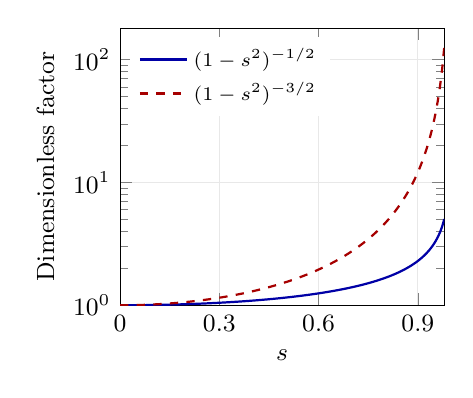
\begin{tikzpicture}
\begin{semilogyaxis}[
 width=0.47\textwidth,height=5.1cm,
 xlabel={$s$},ylabel={Dimensionless factor},
 xmin=0,xmax=0.98,ymin=1,ymax=180,
 xtick={0,0.3,0.6,0.9},ytick={1,10,100},
 tick label style={font=\small},label style={font=\small},
 legend style={font=\scriptsize,at={(0.03,0.97)},anchor=north west,draw=none},
 grid=major,grid style={gray!18}]
\addplot[blue!65!black,thick,domain=0:0.98,samples=150]{1/sqrt(1-x*x)};
\addlegendentry{$(1-s^2)^{-1/2}$}
\addplot[red!65!black,thick,dashed,domain=0:0.98,samples=150]{(1-x*x)^(-1.5)};
\addlegendentry{$(1-s^2)^{-3/2}$}
\end{semilogyaxis}
\end{tikzpicture}\hfill
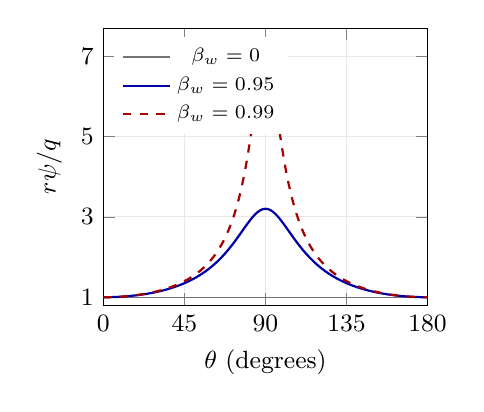
\begin{tikzpicture}
\begin{axis}[
 width=0.47\textwidth,height=5.1cm,
 xlabel={$\theta$ (degrees)},ylabel={$r\psi/q$},
 xmin=0,xmax=180,ymin=0.8,ymax=7.7,
 xtick={0,45,90,135,180},ytick={1,3,5,7},
 tick label style={font=\small},label style={font=\small},
 legend style={font=\scriptsize,at={(0.03,0.97)},anchor=north west,draw=none},
 grid=major,grid style={gray!18}]
\addplot[black!55,domain=0:180,samples=181]{1};
\addlegendentry{$\beta_w=0$}
\addplot[blue!65!black,thick,domain=0:180,samples=181]{1/sqrt(1-0.95*0.95*sin(x)^2)};
\addlegendentry{$\beta_w=0.95$}
\addplot[red!65!black,thick,dashed,domain=0:180,samples=181]{1/sqrt(1-0.99*0.99*sin(x)^2)};
\addlegendentry{$\beta_w=0.99$}
\end{axis}
\end{tikzpicture}
\caption{Analytic illustrations, not experimental data. Left: the common inverse square root and the longitudinal relativistic factor. The acoustic interpretation is only formal near $s=1$, where the linear flow approximation fails. Right: Eq.~\eqref{eq:angular} for the specified coordinate-density scalar source, at fixed present distance $r$. The enhancement is transverse and fore--aft symmetric. These curves are potentials, not gravitational radiation or a force on the source.}
\label{fig:comparison}
\end{figure}

There is a second useful caution. Equation~\eqref{eq:scalar-source} fixes a coordinate density; it is not the source of a Lorentz scalar coupled with invariant proper-time strength. For $c_w=c$, such a covariant scalar source is instead
\begin{equation}
 S_{\rm cov}=4\pi q c\int\delta^{(4)}[x-z(\tau)]\dd\tau
 =\frac{4\pi q}{\gamma}\delta^{(3)}[\bm x-\bm z(t)].
\end{equation}
Its uniform-motion solution is
\begin{equation}
 \psi_{\rm cov}=\frac{q}{\gamma D}
 =\frac{q}{\sqrt{\gamma^2\xi^2+b^2}}.
 \label{eq:cov-scalar}
\end{equation}
The additional $1/\gamma$ changes the amplitude comparison. This is a particularly direct demonstration that finite propagation speed alone does not select a universal enhancement law. One must specify what the source is and how it transforms.

\section{The same calculation for linearized gravity}
\label{sec:gravity}

\subsection{Retarded metric perturbations}

Write $g_{\mu\nu}=\eta_{\mu\nu}+h_{\mu\nu}$ and
$\bar h_{\mu\nu}=h_{\mu\nu}-\eta_{\mu\nu}h/2$. In harmonic gauge, the linearized Einstein equations are~\cite{carroll}
\begin{equation}
 \partial_\mu\bar h^{\mu\nu}=0,\qquad
 \Box\bar h^{\mu\nu}=-\frac{16\pi G}{c^4}T^{\mu\nu},
 \qquad \Box=-c^{-2}\partial_t^2+\nabla^2.
 \label{eq:linear-gr}
\end{equation}
The outgoing solution is
\begin{equation}
 \bar h^{\mu\nu}(t,\bm x)=\frac{4G}{c^4}
 \int\frac{T^{\mu\nu}(t-|\bm x-\bm x'|/c,\bm x')}
 {|\bm x-\bm x'|}\,\dd^3x'.
 \label{eq:ret-gr}
\end{equation}
For a point mass in uniform inertial motion,
\begin{equation}
 T^{\mu\nu}(t,\bm x)=\frac{m u^\mu u^\nu}{\gamma}
 \delta^{(3)}[\bm x-\bm z(t)],
 \qquad u^\mu=\gamma(c,\bm v).
 \label{eq:T-point}
\end{equation}
Applying the same retarded Jacobian gives
\begin{equation}
 \bar h^{\mu\nu}=\frac{4Gm}{c^4}
 \left[\frac{u^\mu u^\nu}{\gamma\kappa R}\right]_{\ret}.
 \label{eq:gr-lw}
\end{equation}
For uniform motion, $\kappa R=D$ from Eq.~\eqref{eq:D} with $c_w=c$, so
\begin{equation}
 \boxed{\bar h^{\mu\nu}=
 \frac{4Gm\,u^\mu u^\nu}{c^4 r'},\qquad
 r'=\sqrt{\gamma^2\xi^2+b^2}.}
 \label{eq:boosted-gr}
\end{equation}
This is exactly the Lorentz transform of the static linearized point-mass field, outside the source. For example, with contravariant indices,
\begin{equation}
 \bar h^{00}=\frac{4Gm\gamma^2}{c^2r'},\quad
 \bar h^{0x}=\frac{4Gm\gamma^2\beta}{c^2r'},\quad
 \bar h^{xx}=\frac{4Gm\gamma^2\beta^2}{c^2r'}.
 \label{eq:metric-components}
\end{equation}
The components can grow substantially with the boost. Yet their spatial denominator is fore--aft symmetric, and the complete solution is a boosted static field, not a radiating wake.

\subsection{Enhancement, coordinate dependence, and radiation}

A stationary laboratory observer and an observer moving with the source can measure different tidal components. Such observer dependence can correspond to real differences in detector response. It does not follow that every large metric component is an invariant strengthening of gravity or a force resisting the source's motion.

For a local freely falling detector, an operational observable is
\begin{equation}
 \mathcal E_{ij}=R_{\hat0 i\hat0 j},\qquad
 \frac{\dd^2 X^i}{\dd\tau_{\rm det}^2}=-c^2\mathcal E^i{}_jX^j,
 \label{eq:tidal}
\end{equation}
where hatted components refer to the detector's orthonormal frame. In linear theory the relevant curvature is constructed from all the metric components:
\begin{equation}
 R_{0i0j}^{(1)}=\frac12\left(
 \partial_0\partial_i h_{0j}+\partial_0\partial_j h_{0i}
 -\partial_i\partial_j h_{00}-\partial_0^2h_{ij}\right).
 \label{eq:curvature}
\end{equation}
Unlike $h_{00}$ alone, the linearized Riemann tensor is invariant under an infinitesimal gauge transformation about Minkowski spacetime. Its projections still depend on the physical observer.

As a complementary check, the leading nonzero weak-field curvature scalar outside a spherical source is
\begin{equation}
 R_{\alpha\beta\gamma\delta}R^{\alpha\beta\gamma\delta}
 =\frac{48G^2m^2}{c^4r'^6}+\Ord(G^3).
 \label{eq:kretschmann}
\end{equation}
At the same spacetime event it is unchanged by a boost. Here $r'$ is the rest-frame radius to leading weak-field order, and the remainder is at fixed $m$ and position. This comparison must not be confused with comparing different events at a fixed laboratory coordinate distance.

Uniform translation of an isolated stationary body produces no outgoing gravitational-wave energy flux. Time dependence at a fixed laboratory location is not sufficient to establish radiation. Conversely, acceleration or changes of the complete system's multipoles can generate radiation; the uniform-motion result does not deny that possibility. The lesson is to calculate a tidal observable, a radiative flux, or a regularized self-force before interpreting component growth as a dynamical barrier.

This also explains why adding a propagation delay to a Newtonian central force is not a consistent shortcut. Velocity-dependent terms and the conservation equations change the result. Carlip's analysis of gravitational aberration provides a closely related example~\cite{carlip}. Equations~\eqref{eq:gr-lw}--\eqref{eq:boosted-gr} make the issue visible without an expansion in $v/c$.

The calculation is first order in $G$, not an unrestricted high-energy approximation. In the chosen laboratory components, a sufficient perturbative condition is $4Gm\gamma^2/(c^2r')\ll1$. An arbitrarily large boost can spoil that componentwise approximation even while rest-frame curvature remains weak. No conclusion about a divergent physical self-force follows by extrapolating these components outside their domain.

\section{What changes when the source accelerates?}
\label{sec:radiation}

\subsection{One must include whatever pushes the body}

The divergence of Eq.~\eqref{eq:linear-gr}, together with harmonic gauge, requires $\partial_\mu T^{\mu\nu}=0$ at the order being used. An arbitrarily prescribed accelerating point mass does not satisfy this requirement by itself. Its covariant distribution is
\begin{equation}
 T_{\rm body}^{\mu\nu}=mc\int u^\mu u^\nu
 \delta^{(4)}[x-z(\tau)]\dd\tau,
\end{equation}
and integration by parts gives
\begin{equation}
 \partial_\mu T_{\rm body}^{\mu\nu}
 =mc\int\frac{\dd u^\nu}{\dd\tau}\delta^{(4)}[x-z(\tau)]\dd\tau.
 \label{eq:nonconserved}
\end{equation}
In a laboratory-time representation this is
$(m/\gamma)(\dd u^\nu/\dd\tau)\delta^{(3)}[\bm x-\bm z(t)]$.
The accelerating agency must supply the opposite divergence. Its fields, reaction mass, supports, or stresses belong in the total source.

This is a physical point rather than a technical obstacle: an object cannot exchange momentum with an unspecified ``push.'' A calculation of gravitational radiation or self-reaction must know where that momentum goes. The body's term in a retarded integral can still be useful, but it is not by itself a complete harmonic-gauge solution for forced motion.

\subsection{Radiation carries a different kind of information}

For a localized, conserved, weak-field source with slow internal motions, let
\begin{equation}
 Q_{ij}(t)=\int\rho(t,\bm x)
 \left(x_i x_j-\frac13\delta_{ij}|\bm x|^2\right)\dd^3x
 \label{eq:quadrupole}
\end{equation}
be its trace-free mass quadrupole. The connection to the source's motion follows directly from conservation: two integrations by parts, with vanishing boundary terms, give
\begin{equation}
 \int T^{ij}\dd^3x
 =\frac{1}{2c^2}\frac{\dd^2}{\dd t^2}
 \int T^{00}x_i x_j\dd^3x
 \simeq\frac12\frac{\dd^2}{\dd t^2}\int\rho x_i x_j\dd^3x.
\end{equation}
In the far-zone, long-wavelength approximation, inserting this identity into Eq.~\eqref{eq:ret-gr} and projecting transverse to the line of sight gives the radiation field. At leading order it and the time-averaged total power are
\begin{align}
 h_{ij}^{\TT}(t,r\bm n)&=\frac{2G}{c^4r}
 \Lambda_{ij,kl}(\bm n)\ddot Q_{kl}(t-r/c),\\
 P_{\rm GW}&=\frac{G}{5c^5}\avg{\dddot Q_{ij}\dddot Q_{ij}}.
 \label{eq:quadrupole-power}
\end{align}
Here $\Lambda_{ij,kl}=P_{ik}P_{jl}-P_{ij}P_{kl}/2$ when acting on a symmetric tensor, with $P_{ij}=\delta_{ij}-n_i n_j$. Repeated spatial indices are summed, and the average is over several cycles for a periodic source. The corresponding wave-zone flux is
\begin{equation}
 \mathcal F_{\rm GW}=\frac{c^3}{32\pi G}
 \avg{\dot h_{ij}^{\TT}\dot h_{ij}^{\TT}}.
 \label{eq:flux}
\end{equation}
Integrating $r^2\mathcal F_{\rm GW}$ over solid angle and using
$\int\!\dd\Omega\,(\Lambda_{ij,kl}B_{kl})^2=(8\pi/5)B_{ij}B_{ij}$ for a symmetric trace-free tensor $B_{ij}$ gives the power in Eq.~\eqref{eq:quadrupole-power}. These formulas concern the radiative $1/r$ field and not an arbitrary time-dependent near-field component~\cite{flanagan}.

For an isolated system, conservation keeps the leading mass monopole constant and gives $\ddot D_i=0$ for the mass dipole $D_i=\int\rho x_i\dd^3x$. This is why the leading radiation is quadrupolar. The derivatives in Eq.~\eqref{eq:quadrupole-power} already show why a rule depending only on a body's instantaneous speed is inadequate. Shape, acceleration history, and the accelerating apparatus affect the answer.

\subsection{A small, explicit example}

Consider two masses in their center-of-mass frame, with reduced mass $\mu$ and separation
\begin{equation}
 \bm r(t)=[L_0+A\cos(\omega t)]\bm e_x.
 \label{eq:dumbbell}
\end{equation}
A weak internal actuator or spring supplies the motion and the stresses needed for total conservation. We assume its mass and energy make a negligible contribution to the \emph{leading Newtonian quadrupole}. This is a slow-motion example, with $\omega L_0/c\ll1$, small compactness, and $A<L_0$; it is not an extrapolation of the quadrupole formula to relativistic internal velocities.

At this order,
\begin{equation}
 Q_{ij}=\mu r^2(t)\,
 \operatorname{diag}(2/3,-1/3,-1/3)_{ij}.
\end{equation}
The elementary calculation in Appendix~\ref{app:dumbbell} yields
\begin{equation}
 \boxed{P_{\rm GW}=\frac{4G\mu^2\omega^6}{15c^5}
 \left(L_0^2A^2+4A^4\right).}
 \label{eq:dumbbell-power}
\end{equation}
For $\mu=1\,\mathrm{kg}$, $L_0=0.1\,\mathrm m$, $A=10^{-3}\,\mathrm m$, and $\omega=2\pi\,\mathrm{s}^{-1}$, this gives
\begin{equation}
 P_{\rm GW}\simeq4.52\times10^{-57}\,\mathrm W.
\end{equation}
This is an analytic estimate for the stated hypothetical system, not a measurement. It illustrates both the smallness of laboratory gravitational radiation and its strong dependence on frequency. At fixed small velocity amplitude $A\omega$, the leading term still changes as $L_0^2\omega^4$. It cannot be represented by a universal factor of $\gamma(v)$.

Radiation reaction is also distinct from a constant mass correction. In a driven periodic system, the cycle-averaged work supplied by the actuator includes the emitted energy. Instantaneously, reversible energy stored in the near field can also change, so $\bm F_{\rm reaction}\cdot\bm v=-P_{\rm GW}$ is not a generally valid instantaneous identity for one selected body.

\section{Can the gravitational field supply the required inertia?}
\label{sec:self-energy}

\subsection{A conservative contribution that can be estimated}

For a weakly self-gravitating body of mass scale $m_0$ and rest-frame radius $\ell$, a natural dimensionless parameter is
\begin{equation}
 \varepsilon_g=\frac{Gm_0}{\ell c^2}\ll1.
 \label{eq:compactness}
\end{equation}
For a uniform Newtonian sphere, assembling shells gives
\begin{equation}
 E_{\rm bind}=-\int_0^\ell\frac{G M(r)}{r}\,\dd M(r)
 =-\frac{3Gm_0^2}{5\ell},\qquad
 \frac{\delta m_g}{m_0}=\frac{E_{\rm bind}}{m_0c^2}
 =-\frac35\varepsilon_g.
 \label{eq:binding}
\end{equation}
The physical mass includes all internal and supporting energy as well as this binding contribution. Consequently Eq.~\eqref{eq:binding} is a simple binding-energy example, not a universal formula for the total mass of every material body.

For $m_0=1\,\mathrm{kg}$ and $\ell=0.1\,\mathrm m$, the compactness is $7.43\times10^{-27}$ and the binding contribution is $\delta m_g/m_0=-4.46\times10^{-27}$. Its sign is negative: gravitational binding does not resemble a positive reservoir of compressed gas. This does not mean that every gravitational dynamical correction must be negative; it means the most immediate conservative estimate is small and has a different interpretation.

\subsection{Why a gravitational correction can contain exactly \texorpdfstring{$\gamma^3$}{gamma cubed}}

Suppose an isolated, stable composite body, including its bound fields and stresses, has invariant rest energy $m_\phys c^2$. Its total four-momentum in an asymptotically inertial frame transforms as
\begin{equation}
 P^\mu=m_\phys u^\mu.
\end{equation}
For adiabatic acceleration that leaves its rest state effectively unchanged and neglects radiative corrections, its force response is therefore
\begin{equation}
 F_\parallel=m_\phys\gamma^3a_\parallel.
\end{equation}
Writing $m_\phys=m_0+\delta m_g$ for the binding contribution under discussion gives
\begin{equation}
 \delta F_\parallel=\delta m_g\gamma^3a_\parallel,
 \qquad
 \frac{\delta F_\parallel}{m_0\gamma^3a_\parallel}
 =\frac{\delta m_g}{m_0}=\Ord(\varepsilon_g).
 \label{eq:delta-force}
\end{equation}
Thus it is quite possible to obtain the \emph{right power} of $\gamma$ in a gravitational contribution. But the power is inherited from the transformation of the total energy--momentum, and the relative contribution in this example remains small. Multiplying a tiny mass correction by $\gamma^3$ does not make it dominate a baseline that contains the same $\gamma^3$.

This is an important distinction for the original association. Matching the dimensions and a divergence pattern is a useful first check, but it does not identify a mechanism. Every ordinary contribution to a stable body's rest energy inherits the same boost law when it belongs to a closed relativistic system. Matching $\gamma^3$ alone cannot single out gravity.

\subsection{Self-force, source size, and a decoupling check}

Evaluating the singular field of a point particle at its own location does not yield a finite physical force. Gravitational self-force theory instead uses a controlled small-body expansion and a regular field, often written schematically as $h^{\ret}=h^{\rm S}+h^{\rm R}$~\cite{poisson}. In a specified background and with a consistent driving system, one can organize the motion schematically as
\begin{equation}
 m_\phys A^\mu=F_{\rm drive}^\mu+
 F_{\rm self}^\mu[h^{\rm R}]+F_{\rm finite\ size}^\mu,
 \label{eq:schematic-self-force}
\end{equation}
where $A^\mu=u^\nu\nabla_\nu u^\mu$, reducing to $\dd u^\mu/\dd\tau$ in inertial flat-spacetime coordinates. This equation indicates the required bookkeeping; it is not a self-force calculation performed in this note. A curved background can produce additional history dependence through propagation inside the light cone.

A straightforward diagnostic is to hold the nongravitational source scales and a subluminal trajectory fixed, and take $G\to0$. Ordinary perturbative gravitational binding and reaction vanish, whereas the special-relativistic relation $F_\parallel=m\gamma^3a_\parallel$ remains. This excludes an explanation in which a regular, weak gravitational self-interaction of that body supplies the entire inertial factor. It does not exclude a different theory with new degrees of freedom, a nonperturbative origin of mass, or cosmological boundary conditions. Such possibilities require additional assumptions, not an extrapolation of the present calculation.

\section{Could spacetime be an effective continuum?}
\label{sec:continuum}

The preceding checks weaken the literal picture of gravity accumulating in front of a body. They leave a broader and more interesting intuition available: perhaps spacetime geometry and the inertia of particles are collective descriptions of some underlying wave-supporting system. This section develops that possibility in two steps. The acoustic and soliton models are calculations within explicitly stated theories. Their interpretation as clues about the vacuum is a conjecture.

\subsection{A calculable bridge: an acoustic spacetime}

In an inviscid, barotropic, irrotational fluid, write a background velocity as $\bm v_0=\bm\nabla\Phi_0$ and perturb the velocity potential by $\varphi$. At linear order, Bernoulli's equation and continuity give
\begin{align}
 \rho_1&=-\frac{\rho_0}{c_s^2}
 (\partial_t+\bm v_0\cdot\bm\nabla)\varphi,\\
 0&=\partial_t\rho_1+
 \bm\nabla\cdot(\rho_1\bm v_0+\rho_0\bm\nabla\varphi).
\end{align}
Eliminating $\rho_1$ yields
\begin{equation}
 \partial_\mu(f^{\mu\nu}\partial_\nu\varphi)=0,
 \qquad
 f^{\mu\nu}=\frac{\rho_0}{c_s^2}
 \begin{pmatrix}
 -1&-v_0^j\\
 -v_0^i&c_s^2\delta^{ij}-v_0^iv_0^j
 \end{pmatrix}.
 \label{eq:acoustic-f}
\end{equation}
In this subsection only, the coordinates are $(t,\bm x)$, rather than $(ct,\bm x)$. In three spatial dimensions, $f^{\mu\nu}=\sqrt{-g_{\rm ac}}\,g_{\rm ac}^{\mu\nu}$ is reproduced by the acoustic line element
\begin{equation}
 \dd s_{\rm ac}^2=\frac{\rho_0}{c_s}
 \left[-(c_s^2-v_0^2)\dd t^2
 -2\bm v_0\cdot\dd\bm x\,\dd t+\dd\bm x^2\right].
 \label{eq:acoustic-metric}
\end{equation}
An overall constant normalization is immaterial. The perturbation therefore obeys the massless scalar wave equation in an effective curved geometry~\cite{barcelo}. This is a precise sense in which a fluid can give rise to a spacetime description for its excitations.

The qualification is equally concrete: $g_{\rm ac}$ is made out of fluid density, velocity, and sound speed. Those variables obey fluid equations, not automatically Einstein's field equations. A scalar sound mode does not reproduce the two tensor polarizations and universal coupling of gravity. The mathematical bridge supports the question, without supplying the missing gravitational dynamics.

\subsection{A wave-supported object with a Lorentz-type inertia}
\label{sec:kink}

An even closer illustration of the inertia intuition is available in a simple one-dimensional continuum. Let a dimensionless field $\phi$ have Lagrangian density
\begin{equation}
 \mathcal L=\frac{\mathcal K}{2c_*^2}\phi_t^2
 -\frac{\mathcal K}{2}\phi_x^2
 -\frac{\mathcal K}{\ell_*^2}(1-\cos\phi),
 \qquad \mathcal K>0.
 \label{eq:sg-action}
\end{equation}
Here $c_*$ is the characteristic speed, $\ell_*$ is a length, and $\mathcal K$ has units of energy times length. The field equation is
\begin{equation}
 c_*^{-2}\phi_{tt}-\phi_{xx}+\ell_*^{-2}\sin\phi=0.
 \label{eq:sg}
\end{equation}
This sine-Gordon model, whose driven soliton dynamics have an established literature~\cite{mclaughlin}, supports the localized kink
\begin{equation}
 \phi_0(x)=4\arctan e^{x/\ell_*},\qquad
 E_0=\frac{8\mathcal K}{\ell_*}.
 \label{eq:kink-static}
\end{equation}
The field interpolates between adjacent vacuum values, while its energy is localized. Substitution verifies that
\begin{equation}
 \phi_v(t,x)=4\arctan\exp\!\left[
 \frac{\gamma_*(x-vt)}{\ell_*}\right],
 \qquad \gamma_*=(1-v^2/c_*^2)^{-1/2},
 \label{eq:kink-moving}
\end{equation}
is an exact uniformly translating solution for $|v|<c_*$.

The conserved energy and momentum follow from the field theory itself:
\begin{align}
 E&=\int\!\dd x\left[
 \frac{\mathcal K}{2c_*^2}\phi_t^2+
 \frac{\mathcal K}{2}\phi_x^2+
 \frac{\mathcal K}{\ell_*^2}(1-\cos\phi)\right],\\
 P&=-\frac{\mathcal K}{c_*^2}\int\phi_t\phi_x\,\dd x.
\end{align}
Using Eq.~\eqref{eq:kink-moving}, or the short integration in Appendix~\ref{app:kink}, gives
\begin{equation}
 \boxed{E=\gamma_*E_0,\qquad
 P=\gamma_*\frac{E_0}{c_*^2}v,\qquad
 \frac{\dd P}{\dd v}=\frac{E_0}{c_*^2}\gamma_*^3.}
 \label{eq:kink-inertia}
\end{equation}
Thus a persistent object made from a wave field can exhibit exactly the same energy and longitudinal-response factors. These are the conserved quantities of this field sector; a material implementation can have additional substrate degrees of freedom. For slow driving that keeps the object close to this family of kinks and produces negligible radiation, $F\simeq(E_0/c_*^2)\gamma_*^3a$. The energy--momentum relation of the uniform family is exact; the accelerated collective-coordinate interpretation is an approximation.

\paragraph{Intuition.}
The ``object'' here is a self-maintaining field profile. Faster motion compresses its spatial structure and increases its field energy (Fig.~\ref{fig:kink}). No gravitational drag or dissipative shock is needed. This is a constructive example of how an inertia law can be expressed in the dynamics of a continuum. Equally, the action~\eqref{eq:sg-action} already has Lorentz symmetry with limiting speed $c_*$. The example does not show that finite propagation alone creates that symmetry, nor that real particles are sine-Gordon kinks. It illustrates a route that is closer to the broad intuition than the forward-pile-up picture is.

\begin{figure}[t]
\centering
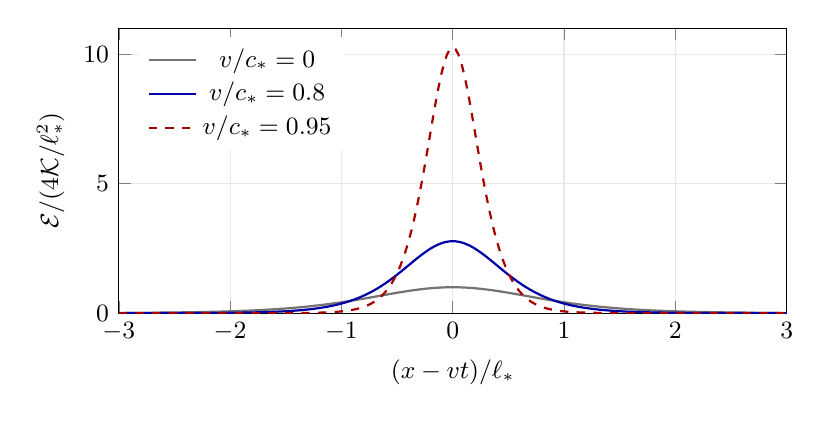
\begin{tikzpicture}
\begin{axis}[
 width=0.83\textwidth,height=5.2cm,
 xlabel={$(x-vt)/\ell_*$},
 ylabel={$\mathcal{E}/(4\mathcal K/\ell_*^2)$},
 xmin=-3,xmax=3,ymin=0,ymax=11,
 tick label style={font=\small},label style={font=\small},
 legend style={font=\small,at={(0.03,0.97)},anchor=north west,draw=none},
 grid=major,grid style={gray!18}]
\addplot[black!55,thick,domain=-3:3,samples=201]{1/(cosh(x)^2)};
\addlegendentry{$v/c_*=0$}
\addplot[blue!65!black,thick,domain=-3:3,samples=201]{(1/0.36)/(cosh(x/0.6)^2)};
\addlegendentry{$v/c_*=0.8$}
\addplot[red!65!black,thick,dashed,domain=-3:3,samples=241]{(1/0.0975)/(cosh(x/sqrt(0.0975))^2)};
\addlegendentry{$v/c_*=0.95$}
\end{axis}
\end{tikzpicture}
\caption{Exact energy-density profiles of the uniformly translating sine-Gordon kink: $\mathcal E=4\mathcal K\gamma_*^2\ell_*^{-2}\operatorname{sech}^2[\gamma_*(x-vt)/\ell_*]$. Increasing speed contracts the profile and increases its integrated energy as $\gamma_*E_0$. This is a continuum-field illustration of relativistic inertia, not a model or measurement of gravitational pile-up.}
\label{fig:kink}
\end{figure}

\subsection{Conjecture: geometry and inertia as collective behavior}

\emph{The following interpretation is speculative.} Suppose the vacuum admits an underlying continuum description, perhaps with microscopic variables quite unlike those of an ordinary liquid. Stable localized excitations could play the role of particles, and their energy together with the surrounding field deformation could determine their inertial mass. The apparent spacetime metric could describe how long-wavelength signals travel through this system. Gravitational disturbances might then be collective excitations of the same substrate rather than waves in an additional material placed inside a pre-existing spacetime.

In that picture, the acoustic resemblance would point to a common causal organization: a localized excitation must evolve consistently with the propagation of its constituent fields. The analogue of the limiting speed would be built into those dynamics. ``Resistance to acceleration'' might be a coarse description of the growing energy required to reshape and transport the excitation, without implying dissipative friction against a preferred medium.

This is a bold possibility, not a consequence of the preceding equations. To become a model of our world, it would have to produce a common low-energy light cone for matter and gravity, a suitable spin-two gravitational sector, the observed equivalence properties, and sufficiently accurate Lorentz symmetry. Neither the acoustic metric nor the scalar kink supplies all of these ingredients. We have not constructed such a theory here. The possibility that the analogy has no deeper connection to the actual vacuum remains entirely plausible, and is the conservative expectation of this note.

\subsection{How the continuum conjecture could acquire predictions}

A microscopic continuum or lattice often introduces an additional length scale. As an illustrative choice, a quadratic effective action in a specified rest frame could contain
\begin{equation}
 \mathcal L_\chi=\frac12\left[
 \dot\chi^2-c_*^2|\bm\nabla\chi|^2
 -c_*^2\ell_{\rm micro}^2(\nabla^2\chi)^2\right].
 \label{eq:dispersion-action}
\end{equation}
For plane waves, direct substitution gives
\begin{align}
 \omega^2&=c_*^2k^2(1+\ell_{\rm micro}^2k^2),\\
 v_{\rm group}&=c_*\left[1+
 \frac32\ell_{\rm micro}^2k^2+
 \Ord(\ell_{\rm micro}^4k^4)\right].
 \label{eq:dispersion}
\end{align}
This is a prediction of the chosen toy action, not a prediction of general relativity or evidence that the vacuum has this dispersion. The higher-spatial-derivative term explicitly selects a frame. The small-$k\ell_{\rm micro}$ expansion does not determine the microscopic front velocity or justify extrapolating to arbitrarily high frequency.

The usefulness of this example is methodological: specifying the underlying dynamics turns ``fluid-like spacetime'' into a question about measurable dispersion, preferred-frame dependence, and whether different species share a limiting speed. A model that reproduces relativity exactly in every accessible observation may provide an interpretation, but not yet a distinguishable physical explanation.

\section{What would turn the idea into a physical test?}
\label{sec:tests}

The preceding examples suggest concrete criteria for a next calculation. A proposed gravitational mechanism should specify an action or closed field equations, the source and its driving agency, boundary conditions, and a measurable response. A useful observable in a prescribed laboratory protocol is the residual
\begin{equation}
 \Delta F_\parallel(t)=F_\parallel(t)
 -m_\phys\gamma^3(t)a_\parallel(t),
 \label{eq:residual}
\end{equation}
after ordinary apparatus effects and other known interactions are accounted for. The rest mass must be independently specified so that a constant binding-energy shift is not counted twice. A calculation that only reproduces the second term is not an additional prediction.

Four comparisons are particularly informative:
\begin{enumerate}
 \item \textbf{Change compactness.} At fixed measured rest mass and controlled drive, vary the body's size or internal distribution. A self-gravitational contribution generally has additional source scales; the ordinary relativistic boost law does not.
 \item \textbf{Change the acceleration history.} Compare protocols with the same instantaneous velocity and acceleration but different earlier motion. Radiative or propagation-memory effects need not agree even when $\gamma$ agrees.
 \item \textbf{Compare frames and force directions.} A viable account must recover the full tensor~\eqref{eq:mass-tensor}, including transverse response, rather than only matching one power of $\gamma$. Any preferred frame introduced by a continuum model must be physically specified and observationally constrained.
 \item \textbf{Measure energy transfer.} A claimed reaction should be consistent with changes of mechanical and bound-field energy and with outgoing radiation. A large potential by itself does not supply this balance.
\end{enumerate}
These are proposed discriminants, not experiments or simulations completed in this work. In the present classical weak-field setting, the estimates above make a laboratory signal from the body's own gravity extremely small.

There is also a closer literal analogue of a wave-speed threshold. If a theory permits a gravitational mode with speed $c_g<c$ in some preferred frame, a sufficiently fast particle could emit gravitational Cherenkov radiation. Moore and Nelson showed that observed high-energy cosmic rays severely constrain such scenarios~\cite{moore}. In general relativity, $c_g=c$ locally and a massive source cannot overtake the gravitational characteristic cone. A genuine gravitational Cherenkov threshold would therefore describe different physics from the standard light-speed limit.

Propagation measurements constrain broader continuum proposals as well. For example, the GW170817/GRB~170817A analysis reported
\begin{equation}
 -3\times10^{-15}\lesssim\frac{c_g-c}{c}
 \lesssim7\times10^{-16},
\end{equation}
under the source-emission timing and propagation assumptions used in that analysis~\cite{abbott}. This is a bound on propagation over that event's observed frequency and distance scales, not a proof about every possible microscopic mode. A conjecture with dispersion or species-dependent speeds must make the corresponding comparison quantitatively.

A final boundary of the analogy deserves mention. General relativity does have an ultrarelativistic shock-like geometry: the Aichelburg--Sexl solution~\cite{aichelburg}. Its limiting construction takes $m\to0$ and $\gamma\to\infty$ at fixed energy $E=\gamma mc^2$. It is not the process of accelerating a fixed-rest-mass body to $c$, and it does not establish a universal drag on that body. A shock-like geometry can be physically meaningful without serving as the explanation sought here.

\section{Discussion and conclusion}

The starting thought can be stated simply: if a moving aircraft has difficulty reorganizing disturbances near the sound speed, might a rapidly moving body experience an analogous difficulty in reorganizing its gravitational field? The calculations make this question more precise without requiring the initial intuition to be correct.

There is a nontrivial mathematical connection. A uniformly translating wave pattern leads to the same anisotropic differential operator that appears in linear compressible flow. Retardation creates angular factors, and a continuum field can support localized excitations whose energy and inertia obey Lorentz-type relations. The acoustic metric and the explicit kink example give the broader ``fluid-like spacetime'' association something firmer than a matching pair of symbols.

The more literal gravitational-pile-up account does not follow. Consistent retardation removes the suggested fore--aft asymmetry for uniform motion in the examples studied. The gravitational solution is a boosted static field, conservative binding renormalizes the rest mass, and radiation depends on the complete evolving system. Within standard weak-field gravity, these effects do not provide an independent origin of the universal $\gamma$ and $\gamma^3$ factors.

The broader conjecture remains open in a different sense: an underlying continuum might produce effective geometry and particle-like excitations together. Here the role of the sound-barrier analogy would be to suggest a common causal structure, rather than a literal wall of gravitational radiation ahead of a particle. Turning that possibility into physics would require a specified theory with the correct gravitational degrees of freedom and a way to distinguish it from existing descriptions. None is supplied by the present note.

It is quite possible that the original association has no deeper bearing on the real vacuum. Even so, tracing it through explicit models is useful: it identifies where the intuition is productive, where it changes meaning, and what would have to be added before it became a testable explanation.

\section*{Author's note and use of AI}
The author is a computer science student, not a professional physicist. This work began as a personal idea pursued in spare time and was developed through discussions with OpenAI's GPT. GPT assisted substantially with mathematical development, literature lookup, organization, and drafting. The paper is intended as an intuitive, exploratory note combining explicit model calculations with clearly identified conjectures. It should not be read as a professionally validated theory or as evidence that the vacuum is a fluid. The AI assistance is disclosed as part of the work's provenance, not as an independent scientific endorsement; responsibility for any submitted version rests with the human author.

\section*{Calculations and reproducibility}
No experimental data or new numerical-relativity results are reported. Both figures are analytic plots of the stated formulas. The accompanying script \texttt{verify\_calculations.py} checks the retarded-time identity, the acoustic metric density, the kink equation and integrated energy--momentum, the quadrupole power, and the numerical estimates. These checks assess mathematical consistency of the specified models; they do not validate the conjectured interpretation of nature.

\appendix
\section{The retarded-time Jacobian}
\label{app:jacobian}

For Eq.~\eqref{eq:wave} with the source~\eqref{eq:scalar-source}, the retarded Green function gives
\begin{equation}
 \psi(t,\bm x)=q\int\frac{
 \delta[t-t'-R(t')/c_w]}{R(t')}\dd t',
 \qquad R(t')=|\bm x-\bm z(t')|.
\end{equation}
Set $f(t')=t-t'-R(t')/c_w$. Since $\dd R/\dd t'=-\bm n\cdot\bm v$, its derivative at the retarded root is
\begin{equation}
 f'(t_r)=-1+\bm n\cdot\bm v(t_r)/c_w=-\kappa.
\end{equation}
For a smooth sub-wave-speed trajectory, $\kappa>0$ and the retarded root is unique when it exists. The delta-function change of variables yields Eq.~\eqref{eq:lw-scalar}. A super-wave-speed medium problem can have multiple roots or an envelope where the Jacobian vanishes; that situation requires separate treatment.

For the uniform sub-wave-speed source, Eq.~\eqref{eq:D} can also be checked directly on the forward axis. At present displacement $\xi=r>0$, one has $R=r/(1-\beta_w)$ and $\kappa=1-\beta_w$. Their product is $r$. The large Jacobian is exactly compensated by the larger retarded distance. Behind the source, $R=r/(1+\beta_w)$ and $\kappa=1+\beta_w$, giving the same product. This one-dimensional check captures why considering the angular factor alone is misleading.

\section{Quadrupole power of the oscillating pair}
\label{app:dumbbell}

In the center-of-mass frame, two point masses have the trace-free quadrupole
\begin{equation}
 Q_{ij}=\mu\left(r_i r_j-\frac13\delta_{ij}r^2\right).
\end{equation}
For Eq.~\eqref{eq:dumbbell}, let $C_{ij}=\operatorname{diag}(2/3,-1/3,-1/3)$, so that $C_{ij}C_{ij}=2/3$. Expanding the squared separation gives
\begin{equation}
 r^2=L_0^2+\frac{A^2}{2}+2L_0A\cos\omega t
 +\frac{A^2}{2}\cos2\omega t.
\end{equation}
Its third derivative is
\begin{equation}
 \frac{\dd^3r^2}{\dd t^3}
 =2L_0A\omega^3\sin\omega t
 +4A^2\omega^3\sin2\omega t.
\end{equation}
Orthogonality of the two harmonics gives
\begin{align}
 \avg{\dddot Q_{ij}\dddot Q_{ij}}
 &=\frac23\mu^2\left(2L_0^2A^2\omega^6+8A^4\omega^6\right)\\
 &=\frac43\mu^2\omega^6(L_0^2A^2+4A^4).
\end{align}
Substitution in Eq.~\eqref{eq:quadrupole-power} yields Eq.~\eqref{eq:dumbbell-power}. The coefficient is exact in $A/L_0$ for the stated sinusoidal trajectory within the leading quadrupole approximation; relativistic, gravitational, and actuator-mass corrections remain outside that approximation.

\section{Kink energy and momentum without a particle ansatz}
\label{app:kink}

For the static profile~\eqref{eq:kink-static},
\begin{equation}
 \phi_0'(\zeta)=\frac{2}{\ell_*}\operatorname{sech}(\zeta/\ell_*),
 \qquad
 \frac{\mathcal K}{2}(\phi_0')^2
 =\frac{\mathcal K}{\ell_*^2}(1-\cos\phi_0).
\end{equation}
Thus $E_0=\mathcal K\int(\phi_0')^2\dd\zeta=8\mathcal K/\ell_*$. For fields with endpoints $\phi(-\infty)=0$ and $\phi(+\infty)=2\pi$, completing the square also gives
\begin{equation}
 E_{\rm static}=\frac{\mathcal K}{2}\int
 \left[\phi_x-\frac{2}{\ell_*}\sin\frac{\phi}{2}\right]^2\dd x
 +\frac{8\mathcal K}{\ell_*}.
\end{equation}
The kink saturates this lower bound, explaining its stability within that sector. For the moving solution, put $\zeta=\gamma_*(x-vt)$, so that $\phi_x=\gamma_*\phi_0'$, $\phi_t=-v\gamma_*\phi_0'$, and $\dd x=\dd\zeta/\gamma_*$. The field equation reduces to the static one because $\gamma_*^2(1-v^2/c_*^2)=1$. The energy integral becomes
\begin{align}
 E&=\frac{\mathcal K}{2\gamma_*}
 \left[\gamma_*^2(1+v^2/c_*^2)+1\right]
 \int(\phi_0')^2\dd\zeta\\
 &=\gamma_* E_0.
\end{align}
Similarly,
\begin{equation}
 P=\frac{\mathcal K v\gamma_*}{c_*^2}
 \int(\phi_0')^2\dd\zeta
 =\gamma_*\frac{E_0}{c_*^2}v.
\end{equation}
Differentiating $\gamma_*v$ gives $\gamma_*^3$, establishing Eq.~\eqref{eq:kink-inertia}. The derivation uses only the specified field action and its solution; its Lorentz symmetry is an input of that action, not a conclusion about the microscopic vacuum.

\clearpage
\begin{thebibliography}{99}

\bibitem{barcelo}
C.~Barcel\'o, S.~Liberati, and M.~Visser,
``Analogue gravity,''
\emph{Living Rev. Relativ.} \textbf{14}, 3 (2011),
\href{https://doi.org/10.12942/lrr-2011-3}{doi:10.12942/lrr-2011-3};
expanded version \href{https://arxiv.org/abs/gr-qc/0505065v4}{arXiv:gr-qc/0505065v4} (2024).

\bibitem{sciama}
D.~W.~Sciama,
``On the origin of inertia,''
\emph{Mon. Not. R. Astron. Soc.} \textbf{113}, 34--42 (1953),
\href{https://doi.org/10.1093/mnras/113.1.34}{doi:10.1093/mnras/113.1.34}.

\bibitem{glauert}
H.~Glauert,
``The effect of compressibility on the lift of an aerofoil,''
\emph{Proc. R. Soc. Lond. A} \textbf{118}, 113--119 (1928),
\href{https://doi.org/10.1098/rspa.1928.0039}{doi:10.1098/rspa.1928.0039}.

\bibitem{mit}
MIT OpenCourseWare,
``Lecture 5: Linear subsonic flow,''
\emph{16.121 Analytical Subsonic Aerodynamics} (Fall 2017),
\href{https://ocw.mit.edu/courses/16-121-analytical-subsonic-aerodynamics-fall-2017/49059b8f1a4532d90aae47c509a93686_MIT16_121F17_lec05.pdf}{lecture notes}.

\bibitem{carroll}
S.~M.~Carroll,
``Lecture notes on general relativity,'' (1997),
\href{https://arxiv.org/abs/gr-qc/9712019}{arXiv:gr-qc/9712019}.

\bibitem{carlip}
S.~Carlip,
``Aberration and the speed of gravity,''
\emph{Phys. Lett. A} \textbf{267}, 81--87 (2000),
\href{https://doi.org/10.1016/S0375-9601(00)00101-8}{doi:10.1016/S0375-9601(00)00101-8},
\href{https://arxiv.org/abs/gr-qc/9909087}{arXiv:gr-qc/9909087}.

\bibitem{flanagan}
\'E.~\'E.~Flanagan and S.~A.~Hughes,
``The basics of gravitational wave theory,''
\emph{New J. Phys.} \textbf{7}, 204 (2005),
\href{https://doi.org/10.1088/1367-2630/7/1/204}{doi:10.1088/1367-2630/7/1/204},
\href{https://arxiv.org/abs/gr-qc/0501041}{arXiv:gr-qc/0501041}.

\bibitem{poisson}
E.~Poisson, A.~Pound, and I.~Vega,
``The motion of point particles in curved spacetime,''
\emph{Living Rev. Relativ.} \textbf{14}, 7 (2011),
\href{https://doi.org/10.12942/lrr-2011-7}{doi:10.12942/lrr-2011-7},
\href{https://arxiv.org/abs/1102.0529}{arXiv:1102.0529}.

\bibitem{mclaughlin}
D.~W.~McLaughlin and A.~C.~Scott,
``Perturbation analysis of fluxon dynamics,''
\emph{Phys. Rev. A} \textbf{18}, 1652--1680 (1978),
\href{https://doi.org/10.1103/PhysRevA.18.1652}{doi:10.1103/PhysRevA.18.1652}.

\bibitem{moore}
G.~D.~Moore and A.~E.~Nelson,
``Lower bound on the propagation speed of gravity from gravitational Cherenkov radiation,''
\emph{J. High Energy Phys.} \textbf{09}, 023 (2001),
\href{https://doi.org/10.1088/1126-6708/2001/09/023}{doi:10.1088/1126-6708/2001/09/023},
\href{https://arxiv.org/abs/hep-ph/0106220}{arXiv:hep-ph/0106220}.

\bibitem{abbott}
B.~P.~Abbott et al. (LIGO Scientific Collaboration, Virgo Collaboration,
Fermi Gamma-Ray Burst Monitor, and INTEGRAL),
``Gravitational waves and gamma-rays from a binary neutron star merger:
GW170817 and GRB 170817A,''
\emph{Astrophys. J. Lett.} \textbf{848}, L13 (2017),
\href{https://doi.org/10.3847/2041-8213/aa920c}{doi:10.3847/2041-8213/aa920c},
\href{https://arxiv.org/abs/1710.05834}{arXiv:1710.05834}.

\bibitem{aichelburg}
P.~C.~Aichelburg and R.~U.~Sexl,
``On the gravitational field of a massless particle,''
\emph{Gen. Relativ. Gravit.} \textbf{2}, 303--312 (1971),
\href{https://doi.org/10.1007/BF00758149}{doi:10.1007/BF00758149}.

\end{thebibliography}
\end{document}
